\documentclass[10pt]{article}
\usepackage{../../local}


\newcommand{\classcode}{Physics 105}
\newcommand{\classname}{Analytic Mechanics}
\renewcommand{\maketitle}{%
\hrule height4pt
\large{Eric Du \hfill \classcode}
\newline
\large{HW 07} \Large{\hfill \classname \hfill} \large{\today}
\hrule height4pt \vskip .7em
\normalsize
}
\linespread{1.1}
\begin{document}
	\maketitle
	\section*{Collaborators}
	I worked with \textbf{Andrew Binder and Adarsh Iyer} to complete this assignment. 

	\section*{Problem 1}
	Derive the moment of inertia tensor of the following objects by explicitly setting up a volume integral
	that circulates $I$. Use symmetry to reduce the number of components you need to consider. 

	\begin{enumerate}[label=\alph*)]
		\item A uniform rod of length $L$. One end of the rod is at the origin, the other end of the rod is at 
			$x = L$, $y = z = 0$.

			\begin{solution}
				For all these problems we use the fact that the moment of inertia is written as:
				\[
					I = \int dm \begin{pmatrix} y^2 + z^2 & -xy & -xz\\
					-xy & x^2 + z^2 & -yz\\ 
					-xz & -yz & x^2 + y^2
				\end{pmatrix} 
				\] 
				In terms of this specific problem, we know that there is no mass in the $y$ and $z$ directions,
				so therefore $I_{xx} = 0$. We also know that due to rotational symmetry, $I_{yy} = I_{zz}$. 
				Further, all off diagonal elements (the products of inertia) are zero due to symmetry. Therefore: 
				\begin{align*}
					I_{yy} = \int_0^L \lambda dx x^2 + z^2 &= \int_0^L \lambda dx x^2 \\
					&= \lambda \frac{L^3}{3} \\
					&= \frac{1}{3}mL^2 
				\end{align*}
				Therefore, the moment of inertia tensor is:
				\[
					I = mL^2 \begin{pmatrix}0 & & \\
					& \frac{1}{3} & \\
					& & \frac{1}{3}\end{pmatrix} 
				\] 
				The off diagonal elements are 0, but I'm just not showing them. 
			\end{solution}
		\item A uniform ball of mass $M$ and radius $R$. The base sits in the $xy$-plane, and the apex points
			upward along the $x$ axis

			\begin{solution}
				Due to symmetry in the problem, we know that $I_{xx} = I_{yy} = I_{zz}$, and $I_{xy} = I_{xz}
				= I_{yz} = 0$. Calculating $I_{xx}$:
				\begin{align*}
					I_{xx} &= \int dm (y^2 + z^2)\\
					&= \rho \int (y^2 + z^2) dV \\
					&= \rho \int_0^R \int_0^{2\pi} \int_0^\pi (r^2 \sin^2 \theta \sin^2 \phi + r^2 \cos^2 \theta)
					r^2 \sin \theta d \theta d\phi dr
				\end{align*}
				Calculating this integral gives:
				\[
					I_{xx} = \frac{8\pi \rho R^5}{15}
				\] 
				then using the fact that $V = \frac{4}{3}\pi R^3$, we get: $I_{xx} = \frac{2}{5}MR^2 = I_{yy}
				= I_{zz}$. Therefore the tensor is: 
				\[
					I = \frac{2}{5}MR^2 \begin{pmatrix} 1 & & \\
					& 1 & \\
					& & 1\end{pmatrix} 
				\] 
			\end{solution}
			\item A uniform cone of mass $M$, height $H$, and base radius $R$. The base sits in the $xy$-plane,
				and the apex points upward along the $z$-axis.

				\begin{solution}
					Here, along the $x$ and $y$ axis there is symmetry, so therefore $I_{xy} = I_{xz} = I_{yz} 
					= 0$. Furthermore, we have $I_{yy} = I_{xx}$ due to the same symmetry. Integrating using 
					cylindrical coordinates (I'm going to skip a lot of the algebra):
					\begin{align*}
						I_{zz} &= \rho \int_0^H \int_0^{R\left( 1 - \frac{z}{H} \right)} \int_0^{2\pi} (r^2 \cos 
							\theta + r^2 \sin^2 \theta) r d \theta dr dz\\
							&= 2\pi \rho \int_0^H \int_0^{R\left( 1 - \frac{z}{H} \right)} r^3 dr dz \\
							&= \frac{\pi \rho R^4}{2}\int_0^H \left( 1 - \frac{z}{H} \right)^4 dz\\
							&= \frac{\pi \rho R^4}{2}\int_1^0 (-H) u^4 du \\
							&= \frac{\pi \rho R^4H}{10}
					\end{align*}
					Using the fact that the mass of a cone is $M = \frac{1}{3}\pi R^2 H \rho$, we get: 
					\[
					 I_{zz} = \frac{3}{10}MR^2
					\] 
					Now for $I_{yy}$ (again, I'm going to just set up the integral and skip to nearly the final
					step):
					\begin{align*}
						I_{yy} &= \rho \int dV (x^2 + z^2)\\
							   &= \rho \int_0^H \int_0^{R\left( 1 - \frac{z}{H} \right) } \int_0^{2\pi}
							   (r^2 \cos^2 \theta + z^2)r d \theta dr dz\\
							   &= \pi \rho R^2 \int_0^H \frac{R^2}{4}\left( 1 - \frac{z}{H} \right)^4 + z^2
							   \left( 1 - \frac{z}{H} \right)^2\\
							   &= \pi \rho \frac{R^4}{4} \int_1^0 u^4(-H) du + \pi \rho R^2 \int_0^H z^2
							   \left( 1 - \frac{z}{H} \right)^2\\
							   &= \frac{\pi \rho R^4H}{20} + \frac{\pi \rho R^2H^3}{30}\\
							   &= \frac{3}{20}MR^2 + \frac{1}{10}MR^2H^2 
					\end{align*}
					Therefore, the moment of inertia tensor is: 
					\[
						I = \begin{pmatrix} \frac{3}{10}MR^2 & & \\
						& \frac{3}{20}MR^2 + \frac{1}{10}MR^2H^2& \\
						& & \frac{3}{20}MR^2 + \frac{1}{10}MR^2 H^2 \end{pmatrix} 
					\] 
				\end{solution}
			\item A uniform rectangular prism with mass $M$ and with side lengths $a, b$ and $c$, with one corner
				at the origin, and each side along one of the coordinate axes.

				\begin{solution}
					Here, we have to take all integrals because there is no symmetry in the problem. Thankfully,
					the integrals are quite easy:
					\begin{align*}
						I_{xx} &= \int dm (y^2 + z^2)\\
						&= \rho \int_0^a \int_0^b \int_0^c (y^2 + z^2) dz dy dx \\
						&= \rho a \int_0^b \int_0^c y^2 + z^2 dz dy  \\
						&= \rho a\left( \frac{b^3c}{3} + \frac{c^3b}{3} \right)  \\
						&= \frac{M}{3}(b^2 + c^2) 
					\end{align*}
					Note that we have a pattern here: we square the sides that we're integrating, and omit the 
					one we're not integrating over. Therefore:
					\begin{align*}
						I_{yy} &= \frac{M}{3}(a^2 + c^2) & I_{zz} &= \frac{M}{3}(a^2 + b^2)
					\end{align*}
					Now calculating $I_{xy}$:
					\begin{align*}
						I_{xy} &= -\int dm (xy) = \rho \int_0^a \int_0^b \int_0^c xy dz dy dx\\
						&= -\rho c \int_0^a \int 0^b xy dy dx \\
						&= -\rho c\int_0^a \frac{b^2}{2}x dx \\
						&= -\rho c \frac{b^2 a^2}{4} \\
						&= -\frac{M}{4}(ab) 
					\end{align*}
					Therefore, the other two (just by looking at the pattern):
					\begin{align*}
						I_{yz} &=- \frac{M}{4}(bc) & I_{xz} &=- \frac{M}{4}(ac)
					\end{align*}
					Putting together the matrix, we get:
					\[
						I =M \begin{pmatrix} \frac{1}{3}(b^2 + c^2) &- \frac{1}{4}ab & -\frac{1}{4}ac \\
							-\frac{1}{4}ab & (a^2 + c^2) & -\frac{1}{4}bc\\
							-\frac{1}{4}ac& - \frac{1}{4}bc & \frac{1}{3}(a^2 + b^2)
						\end{pmatrix} 
					\] 
				\end{solution}
	\end{enumerate}

	\pagebreak
	\section*{Problem 2}

	A rigid body consists of three equal masses, $m$, fastened at the positions $(a, 0, 0)$, $(0, a, 2a)$, and
	$(0, a, 2a)$. 
	\begin{enumerate}[label=\alph*)]
		\item Find the inertia tensor $I$

			\begin{solution}
				In the case of discrete masses, the moment of inertia tensor is: 
				\[
					I = \sum_{i = 1}^n m_i \begin{pmatrix} y_{i}^2 + z_i^2 & -x_{i}y_{i}& -x_{i}z_i\\
					-x_{i}y_{i} & x_{i}^2 + z_i^2 &- y_{i}z_i\\
					-x_{i}z_i & -y_iz_i & x_{i}^2y_{i}^2
				\end{pmatrix} 
				\] 
				Therefore, calculating these values, we get:
				\begin{align*}
					I_{xx} &= m(a^2 + 4a^2) + m(4a^2 + a^2) = 10ma^2\\
					I_{yy} &= m(a^2) + m(4a^2) + m(a^2) = 6ma^2 \\
					I_{zz} &=  m(a^2) + m(a^2) + m(4a^2) = 6ma^2 
				\end{align*}
				Further, since in all the masses have either one of $x$ or $y$ being zero, then $I_{xy} = 
				I_{xz} = 0$. Calculating $I_{yz}$, we get:
				\[
					I_{yz} = -m(0) - m(2a^2) - m(2a^2) = -4ma^2
				\] 
				Therefore, the inertia tensor is: 
				\[
					I = ma^2 \begin{pmatrix} 10 & 0 & 0\\
					0 & 6 & -4\\
					0 & -4 & 6\end{pmatrix} 
				\] 
			\end{solution}
		\item Find the principal moments and set of orthogonal principal axes.

			\begin{solution}
				To find the principal moments, we diagonalize this matrix and find the eigenvectors. Doing so, 
				we get:
				\[
					I = ma^2 \begin{pmatrix} 10 & 0 & 0\\
					0 & 10 & 0\\
					0 & 0 & 2
				\end{pmatrix} 
				\] 
				These are the moments of inertia about the principal axes. The eigenvectors are: 
				\begin{align*}
					\omega_1 &= \begin{pmatrix} 1\\0\\0 \end{pmatrix} & \omega_2 &= \begin{pmatrix} 0 \\ -1 \\ 1
				\end{pmatrix} & \omega_3 = \begin{pmatrix} 0\\1 \\1 \end{pmatrix} 
				\end{align*}
				which are the principal axes of motion. 
			\end{solution}
	\end{enumerate}
	\pagebreak
	\section*{Problem 3}
	Let's say you have a cube of mass $M$ and sidelength $L$. Consider three situations: rotating the cube with 
	angular frequency $\omega$ about an axis defined by two points on the cube: (i) two opposite corners; (ii)
	midpoints on two opposite edges; (iii) centers of two opposite faces. In which case is the kinetic 
	energy the largest? The smallest? Of if some cases are equal, indicate that. 

	\begin{solution}
		Here, note that all three rotation axes pass through the center of the cube. We know that due to 
		symmetry, the moment of inertia tensor is actually the identity, so the rotational kinetic energy:
		\[ T_R = \frac{1}{2}I \omega^2\]
		Therefore, the moment of inertia of all three actually just drop out of the calculation, meaning that 
		there is actually no difference in the moments of inertia for all three cases! Therefore, they all
		have the same kinetic energy. 
	\end{solution}

	\pagebreak
	\section*{Problem 4}
	A disk of mass $M$ and radius $R$ unwinds from a tape wrapped around it (see figure below). The tape passes
	over a frictionless pulley, and a mass $m$ is suspended from the other end. Assume the disk drops vertically.

	\begin{center}
		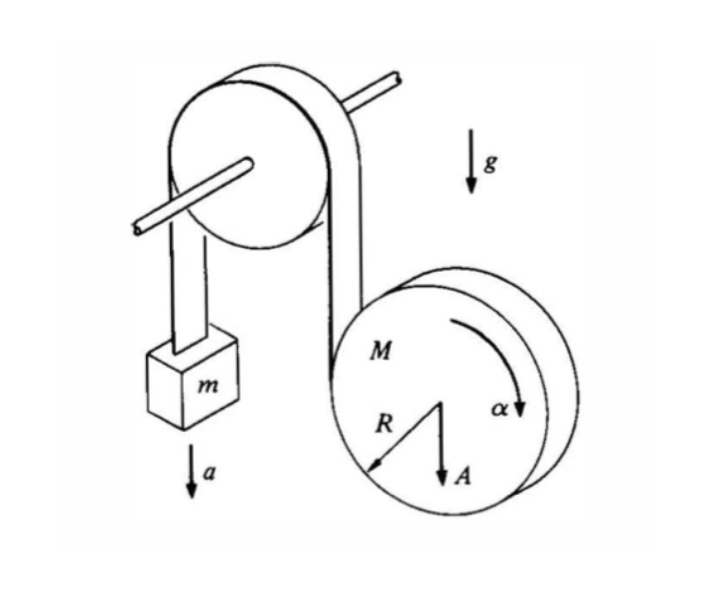
\includegraphics[scale=0.8]{q3.png}
	\end{center}
	\begin{enumerate}[label=\alph*)]
		\item Relate the accelerations of $m$ and $M$, $a$ and $A$, respectively, to the angular acceleration of
			the disk, $\alpha$. \textit{Check: If $A = 2A$, then $\alpha = 3A/R$}

			\begin{solution}
				This comes from the constraint equation. Let $x$ be the difference in height between the top
				of the pulley and the mass $m$, let $y$ be the same difference but with the roll of tape $M$.
				Further, let $\theta$ be the angle that the tape turns. Therefore, the correct constraint is: 
				\[
				x + y = l + R \theta
				\] 
				where $l$ represents the initial length of rope, which is a constant. Taking the second 
				derivative, we get: 
				\[
				\ddot x + \ddot y = R\alpha \implies \alpha = \frac{a + A}{R}
				\] 
				This also passes our check, since $A = 2a$, we do get $\alpha = \frac{3a}{R}$
			\end{solution}
		\item Find $a$, $A$ and $\alpha$.

			\begin{solution}
				Writing down the equations of motion (in Newtonian form), we have; 
				\begin{align*}
					mg - T &= ma \\
					Mg - T &= MA 
				\end{align*}
				The torque on the system is supplied by $T$ which is $T = I \alpha$, and using the moment of 
				inertia of a disc, we have:
				\[
				T = \frac{1}{2}MR^2 \alpha
				\] 
				Substituting this equation and also $\alpha$ into the equations of motion, we get:
				\begin{align*}
					mg - \frac{1}{2}MR^2 \left(\frac{a + A}{R}\right) &= ma\\
					Mg - \frac{1}{2}MR^2 \left(\frac{a + A}{R}\right) &= MA
				\end{align*}
				Solving for $a$ and $A$, which is just a lot of algebra, we get:
				\begin{align*}
					a &= \left( \frac{3m - M}{3m + M} \right) g\\
					A &= \left( \frac{m + M}{3m+M} \right) g \\
					\alpha &= \frac{4mg}{(3m + M)R}
				\end{align*}
			\end{solution}
	\end{enumerate}

	\pagebreak
	\section*{Problem 5}
	A gyroscope is at one end of an axle of length $l$. The other end of the axle is suspended from a string 
	of length $L$. The wheel is set into motion so that it executes uniform precession in the horizontal plane
	due to a weak torque caused by gravity (which points downwards in the figure). The gyroscope is a solid disk
	of mass $M$ and radius $R$, its spin angular velocity is $\omega_s$. Neglect the mass of the shaft and of the
	string. Find the angle $\beta$ that the string with the vertical. Assume $\beta$ is small. 

	\begin{center}
		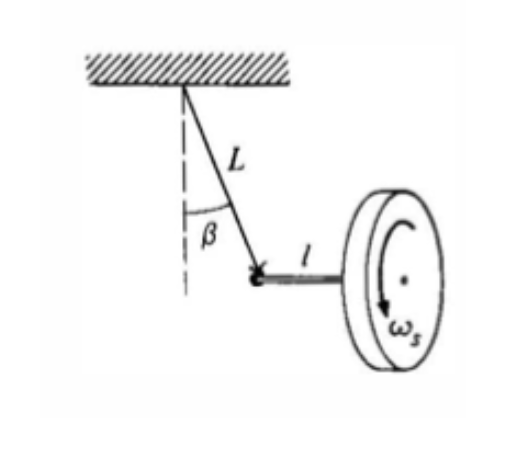
\includegraphics[scale=0.8]{q5.png}
	\end{center}

	
	\begin{solution}
		There is tension in the string, we have: 
		\begin{align*}
			T \cos \beta &= Mg  \\
			T \sin \beta &= M\Omega^2 (l + L \sin \beta)
		\end{align*}
		Using the small angle approximations, we get:
		\begin{align*}
			T &= Mg \\
			T \beta &= M\Omega^2(l + L\beta)
		\end{align*}
		Plugging the second into the first we get:
		\begin{align*}
			Mg\beta &= m\Omega^2 (l + L\beta) \\
			\therefore \beta &= \frac{\Omega^2 l}{g - \Omega^2 L}	
		\end{align*}
		Now, all we need to solve for is $\Omega$ and we solve the problem. Recall from lecture that we have
		\[
		\Omega = \frac{MgR}{\lambda_3 \omega}\hat{z}
		\] 
		Replacing $R = l$ in our situation, we get 
		\[
			\Omega = \frac{Mgl}{\lambda_3 \omega_s}
		\]
		Further, we know $\lambda_3$ since the disk is spinning about its
		principal axis, which we know is $\frac{1}{2}MR^2$ (this is a
		relatively well known result). Therefore, 
		\[
		\Omega = \frac{2gl}{R^2 \omega_s}
		\] 
		Therefore, substituting this back into the expression for $\beta$, we get:
		\begin{align*}
			\beta &= \frac{\left( \frac{2gl}{R^2 \omega_s} \right)^2 l}{g - \left( \frac{2gl}{R^2 \omega_s}
			\right)^2 L} \\
			&= \frac{4gl^3}{R^2 \omega_s^2 - 4gl^2L}
		\end{align*}
	\end{solution}

\end{document}
